\chapter{Location-based Games} 
%\label{sec:}
\section{Hintergrund}
Im folgenden Kapitel wird erläutert was genau ein Location-based Game ausmacht, welche möglichen Spielszenarien es gibt und wie diese funktionieren. Bei Location-based Games handelt es sich um Spiele die zusätzlich zu den Eingaben des Spielers dessen geographische Position mit in das Spiel einbeziehen. So haben Spieler die Möglichkeit Elemente in einem Spiel durch ihren aktuellen Aufenthaltsort oder durch Änderung dieses Ortes zu beeinflussen. Die Positionsdaten werden hierbei meist per GPS ermittelt. Da nahezu alle aktuellen Smartphones ein GPS-Modul besitzen, eignen sie sich perfekt als mobile LBG-Spielekonsole.
 
\section{Mögliche Spielszenarien} 
%\label{sec:}
In einem LBG können grundsätzlich vier verschiedene Spielszenarien umgesetzt werden. Im Folgenden werden diese Szenarien sowohl textuell als auch graphisch beschrieben. 
In den \textbf{Abbildungen \ref{szenA}} bis \textbf{\ref{szenD}} ist der Spieler als grüner Punkt, sein Ziel als roter Punkt und der Weg dorthin als grauer Pfeil gekennzeichnet. In zwei Abbildungen wird ein zeitlicher Ablauf dargestellt. Dies geschieht über den Grad der Verschwommenheit. Je verschwommener eine Graphik ist, desto weiter liegt sie in der Vergangenheit.

\subsection{Versteckspiel} 
\label{sec:szenarioVerstecken}

Angelehnt an das Kinderspiel Verstecken, hat dieses Szenario das Ziel einen Gegenstand, ein Gebäude oder ein Gebiet an einer fixen Postion zu finden. Der Weg dorthin kann auf unterschiedliche Arten beschrieben werden. So ist möglich den Spieler per Navigation zu diesem Punkt zu führen oder ihm lediglich die Koordinaten der Postion mitzuteilen. Ein Pfeil der in die richtige Richtung zeigt oder ein Objekt auf dem Bildschirm, das die Farbe ändert, je nachdem ob er sich dem Ziel nähert oder sich davon entfernt wäre auch denkbar. Eine Umsetzung hiervon ist das sog. Geocaching, bei dem Spieler durch Hinweise und ungefähre Ortsangaben Gegenstände finden müssen.
\cite{Dyer:2010wt}


\begin{figure}[h]
    \centering
    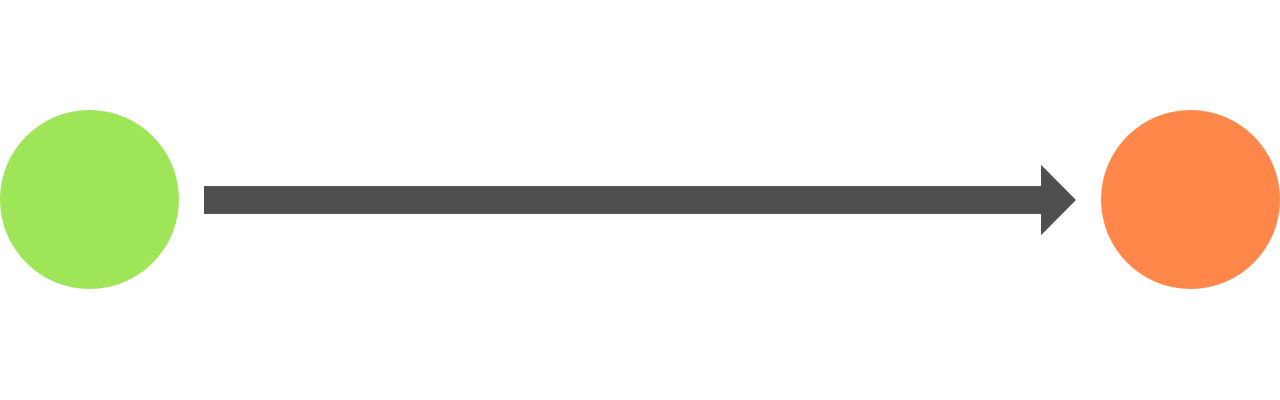
\includegraphics[width=.8\textwidth]{files/lbgArten/searchAndFind}
    \caption{Veranschaulichung des Versteckspielszenarios}
    \label{szenA}
\end{figure}

\subsection{Folge dem Pfad} 
%\label{sec:}

Diese Variante hat Ähnlichkeiten mit einem Rennen. Ziel des Spielers ist es einer vorgegebenen Route zu folgen. Die Routen können hierbei vom Entwickler oder anderen Spielern erstellt werden. Diverse Jogging-Apps arbeiten auf diesem Prinzip. Läufer A läuft eine bestimmte Strecke, speichert sie und andere Läufer haben dann die Möglichkeit sich mit Läufer A zu messen. Wie mit Abweichungen der definierten Route umgegangen wird muss vorher überlegt werden. Bei einer Jogging-App wäre es sinnvoll Strafpunkte für die Größe der Abweichung zu verteilen. Bei anderen Apps, wäre es evtl. sinnvoller die neue Route anders auszuwerten, um so alternativ Routen anzubieten.   Zusätzlich können auch alle Elemente des Versteckspiels, wie in Abschnitt \ref{sec:verstecken} beschrieben, genutzt werden. So kann auch hier die Route auf verschiedenste Arten beschrieben werden und am Ziel das ein bestimmten Objektes sein. 
\cite{creativeworklineGmbH:vb}


\begin{figure}[h]
    \centering
    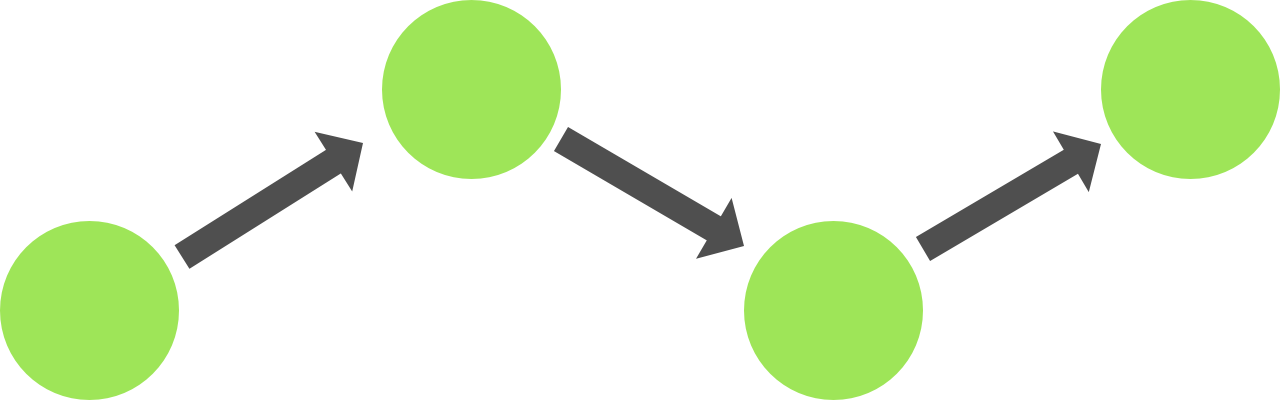
\includegraphics[width=.8\textwidth]{files/lbgArten/followThePath}
    \caption{Veranschaulichung des Folge dem Pfad Szenarios}
    \label{szenB}
\end{figure}


\subsection{Fangen} 
\label{sec:szenarioFangen}
Das häufig von Grund- und Vorschulkindern gespielte Spiel Fangen kann auch im Location-based Rahmen umgesetzt werden. Die Aufgabe des Spielers ist es ein sich bewegendes Objekt in der Spielwelt zu fangen. Zu diesen Objekten können andere Spieler gehören, was die Ähnlichkeit zum Kinderspiel nahe legt oder ein virtuelles Objekt. Der entscheidende Punkt hierbei ist die Bewegung des Objektes. Durch verschiedene Bewegungsmuster muss der Spieler unterschiedliche Strategien entwickeln. Bewegt sich ein Objekt z.B. im Kreis, hat der Spieler die Möglichkeit abzukürzen. Zusätzlich spielt das Intervall, in dem sich das Objekt bewegt eine weitere wichtige Rolle bei der Entwicklung der Fangstrategien.
\cite{Misund:2009ge}

\begin{figure}[h]
    \centering
    
\includegraphics[width=.8\textwidth]{files/lbgArten/chaseAndCatch}
    \caption{Veranschaulichung des Szenarios Fangen}
    %\label{chart:alterFreizeit}
\end{figure}

\subsection{Positionsänderungen} 
\label{sec:szenarioPosition}
Im Gegensatz zu den drei anderen vorgestellten Szenarien ist es hier nicht von Bedeutung ein bestimmtes Ziel zu erreichen. Auch das Einhalten einer vorgegeben Route muss nicht berücksichtigt werden. Es geht viel mehr darum, dass der Spieler sich bewegt. Am ehesten lässt sich dies mit einem Spaziergang mit einem Haustier vergleichen. Auch hier kommt es nicht auf ein Ziel oder die gewählte Route an. Lediglich die Geschwindigkeit mit der sich ein Spieler bewegt, kann hierbei berücksichtigt werden. 
Das Spiel The Journey der Firma Mopius benutzt dieses Prinzip. Dem Spieler entfaltet sich die Geschichte des Spiels umso mehr, je weiter er sich fortbewegt.
\cite{mopius:PZPdJF8n}

\begin{figure}[h]
    \centering
    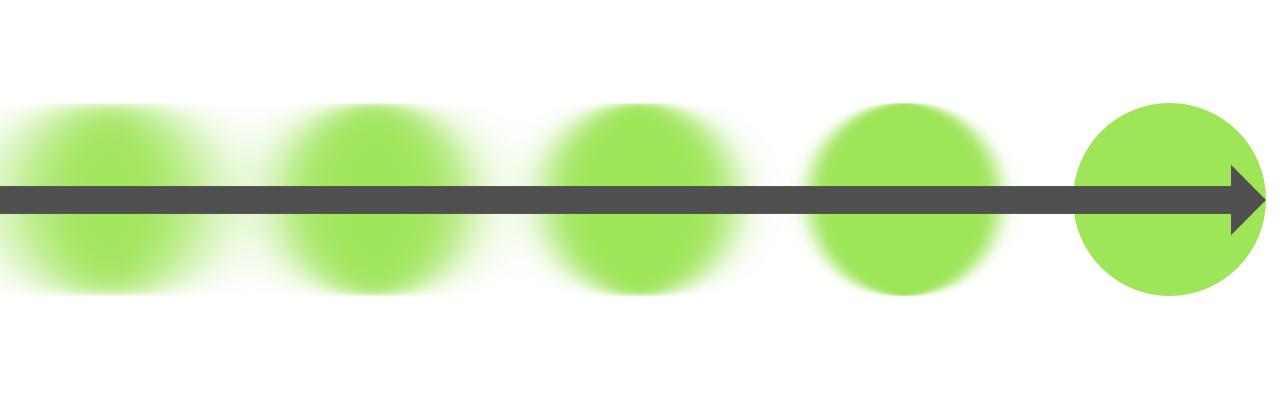
\includegraphics[width=.8\textwidth]{files/lbgArten/changeOfDistance}
    \caption{Veranschaulichung des Szenarios Positionsänderung}
    \label{szenD}
\end{figure}

\section{Verfügbare Spiele und Spielkonzepte} 
%\label{sec:}

\subsection{Mobbles} 
%\label{sec:}
Mobbles ist im Mai 2012 erschienen. In den ersten Versionen war es lediglich möglich verschiedene Mobbles zu fangen, die auf einer Karte in der Umgebung des Spielers angezeigt wurden. Des Weiteren war es möglich die gefangenen virtuellen Tiere mit Freunden zu tauschen. Neben dem Sammelaspekt gab es auch noch die Möglichkeit die gefangenen Mobbles zu umsorgen. Hierbei standen dem Spieler diverse Nahrungsmittel sowie kosmetische Gegenstände, die nur das Aussehen des Tieres ändern zur Verfügung. Seit Mai 2013 ist es aber auch möglich gegen die Mobbles anderer Spieler zu kämpfen. Als Kampfsystem dient hierbei ein einfaches Schere-Stein-Papier-Spiel.  

Spiel basiert auf \ref{sec:szenarioVerstecken}

\subsection{ShadowCities} 
%\label{sec:}
ShadowCites wurde im November 2010 veröffentlich und ist seit Oktober 2013 nicht mehr verfügbar. Es handelte sich bei diesem Spiel um ein MMORPG. Aufgabe des Spielers war es gegen andere Spieler zu kämpfen und Gebiete für seine Fraktion einzunehmen. Das Kampfsystem ist so aufgebaut, dass ein Spieler einen anderen Spieler, der sich in Reichweite befindet auf der Karte antippt und danach einen sog. Zauber per Gestensteuerung auf ihn wirkt. Auch der Bau von Energieknoten, die zum Spielen benötigt werden können so mit anderen Gesten platziert werden. 

Spiel basiert auf \ref{sec:szenarioFangen}

Ähnlichkeiten zu Ingress


\subsection{The Journey} 
%\label{sec:}
The Journey ist genau genommen kein Spiel sondern lediglich eine Geschichte, deren Kapitel durch Spaziergänge freigeschaltet werden können. 

\ref{sec:szenarioPosition}

\chapter{Æthershards} 
%\label{sec:}
\section{Grundlagen} 
%\label{sec:}

Æthershards ist ein seit Sommer 2012 sich in der Entwicklung befindendes Spielkonzept für ein LBG. In der Grundversion überschneidet mit dem Grundgedanken von Mobbles. Denn auch in diesem Spiel ist es die Hauptaufgabe verschiedene virtuelle Haustiere zu fangen und sich anschließend um diese zu kümmern. 

- weitere Eckpunkte aus der PA übernehmen

%\subsection{Technischer Hintergrund}
%\label{sec:techHintergrund}
%Im folgenden Abschnitt wird erläutert, wie Position eines Spielers ermittelt werden kann \textbf{Ortung per GPS}:\\
%1. Satelliten im Weltraum\\
%2. Bodenstationen als Kontroll-Segment\\
%3. geostationäre Satelliten mit Korrektursignalen und\\
%4. das GPS Gerät des Benutzers.


%\subsubsection{Risiken}
%\label{sec:problemstellungen}
%Durch Location-based Games stellten sich entsprechende neue Herausforderungen, die von den jeweiligen Spielen gemeistert werden müssen, raus. Durch die wachsende Popularität und stetig zunehmende Anzahl von Caches, werden die Spieler immer kreativer und suchen Orte die immer schwieriger zu erreichen sind. So werden Caches unter Brücken angebracht, auf der Spitze von Türmen, in Seen usw. Dies führte unweigerlich dazu, dass Spieler auch immer wieder in Konflikt mit dem Gesetz geraten sind. Ein einfaches Beispiel wäre hierzu ein Cache der mitten auf einem Acker vergraben ist. Je nach Saison ist dieser aber bestellt. Was zur Folge haben kann, das mindestens ein oder mehrere Spieler, um den Cache zu haben, den Acker betreten und unweigerlich Pflanzen und somit Eigentum des Bauern zerstören. 
%Der andere kritische Punkt sind gefahren Bereiche. Auch hier soll ein Beispiel zur Verdeutlichung helfen. Der Mittelstreifen einer Autobahn ist für gewöhnlich nicht erreichbar, trotzdem wurden auch schon dort Caches versteckt. Dies ist natürlich ein großes Problem, da gerade Kinder und Jugendliche solche Spiele spielen, ist es schwierig sie davor abzuhalten, solche Caches schon als eine Art Mutprobe angesehen werden können. 
